\documentclass{article}

% Hier befinden sich Pakete, die wir beinahe immer benutzen ...

\usepackage[utf8]{inputenc}

% Sprach-Paket:
\usepackage[english]{babel}

% damit's nicht so, wie beim Grill aussieht:
\usepackage{fullpage}
\usepackage{changepage}

% Mathematik:
\usepackage{amsmath, amssymb, amsfonts, amsthm}
\usepackage{bbm, mathrsfs, stmaryrd}
\usepackage{mathtools, mathdots}

% Doppel-Klammern:
\usepackage{stmaryrd}

% Makros mit mehereren Default-Argumenten:
\usepackage{twoopt}

% Anführungszeichen (Makro \Quote{}):
\usepackage{babel}

% if's für Makros:
\usepackage{xifthen}
\usepackage{etoolbox}

% *'s für Makros:
\usepackage{suffix}

% tikz ist kein Zeichenprogramm (doch!):
\usepackage{tikz}
\usetikzlibrary{arrows}
\usetikzlibrary{decorations.markings}

% bessere Aufzählungen:
\usepackage{enumitem}

% (bessere) Umgebung für Bilder:
\usepackage{graphicx, subfig, float}
\usepackage{tcolorbox}

% Umgebung für Code:
\usepackage{listings}

% Farben:
\usepackage{xcolor}

% Umgebung für "plain text":
\usepackage{verbatim}

% Umgebung für mehrerer Spalten:
\usepackage{multicol}
\setlength{\columnsep}{1cm}

% diagonale Brüche
\usepackage{nicefrac}

% faktorisieren
\usepackage{faktor}

% Spaltentypen verschiedener Dicke
\usepackage{tabularx}
\usepackage{makecell}

% Für Vektoren
\usepackage{esvect}

% (Web-)Links
\usepackage{hyperref}

% Zitieren & Literatur-Verzeichnis
\usepackage[
backend=biber,
style=numeric
]{biblatex}
\usepackage{csquotes}

% so ähnlich wie mathbb
%\usepackage{mathds}

% Keine Ahnung, was das macht ...
\usepackage{booktabs}
\usepackage{ngerman}
\usepackage{placeins}

% Bäume
\usepackage[noeepic]{qtree}

% Algorithmen
\usepackage{algorithm}
\usepackage{algpseudocode}

% ---------------------------------------------------------------- %
% special letters

\newcommand{\N}{\mathbb N}
\newcommand{\Z}{\mathbb Z}
\newcommand{\Q}{\mathbb Q}
\newcommand{\R}{\mathbb R}
\newcommand{\C}{\mathbb C}
\newcommand{\K}{\mathbb K}
\newcommand{\T}{\mathbb T}
\newcommand{\E}{\mathbb E}
\newcommand{\V}{\mathbb V}
\renewcommand{\S}{\mathbb S}
\renewcommand{\P}{\mathbb P}
\newcommand{\1}{\mathbbm 1}
\newcommand{\G}{\mathbb G}

\newcommand{\iu}{\mathrm i}

% ---------------------------------------------------------------- %
% quantors

\newcommand{\Forall}        {\forall ~}
\newcommand{\Exists}        {\exists ~}
\newcommand{\nExists}       {\nexists ~}
\newcommand{\ExistsOnlyOne} {\exists! ~}
\newcommand{\nExistsOnlyOne}{\nexists! ~}
\newcommand{\ForAlmostAll}  {\forall^\infty ~}

% ---------------------------------------------------------------- %
% graphics boxed

\newcommand
{\includegraphicsboxed}
[2][0.75]
{
    \begin{center}
        \begin{tcolorbox}[standard jigsaw, opacityback = 0]

            \centering
            \includegraphics[width = #1 \textwidth]{#2}

        \end{tcolorbox}
    \end{center}
}

\newcommand
{\includegraphicsunboxed}
[2][0.75]
{
    \begin{center}
        \includegraphics[width = #1 \textwidth]{#2}
    \end{center}
}

\NewDocumentCommand
{\includegraphicsgraphicsboxed}
{ O{0.75} O{0.25} m m}
{
    \begin{center}
        \begin{tcolorbox}[standard jigsaw, opacityback = 0]

            \centering
            \includegraphics[width = #1 \textwidth]{#3} \\
            \vspace{#2 cm}
            \includegraphics[width = #1 \textwidth]{#4}

        \end{tcolorbox}
    \end{center}
}

\NewDocumentCommand
{\includegraphicsgraphicsunboxed}
{ O{0.75} O{0.25} m m}
{
    \begin{center}

        \centering
        \includegraphics[width = #1 \textwidth]{#3} \\
        \vspace{#2 cm}
        \includegraphics[width = #1 \textwidth]{#4}

    \end{center}
}

% ---------------------------------------------------------------- %
% braces

\newcommand{\pbraces}[1]{{\left  ( #1 \right  )}}
\newcommand{\bbraces}[1]{{\left  [ #1 \right  ]}}
\newcommand{\Bbraces}[1]{{\left \{ #1 \right \}}}
\newcommand{\vbraces}[1]{{\left  | #1 \right  |}}
\newcommand{\Vbraces}[1]{{\left \| #1 \right \|}}

\newcommand{\abraces}[1]{{\left \langle #1 \right \rangle}}

\newcommand{\floorbraces}[1]{{\left \lfloor #1 \right \rfloor}}
\newcommand{\ceilbraces} [1]{{\left \lceil  #1 \right \rceil }}

\newcommand{\dbbraces}    [1]{{\llbracket     #1 \rrbracket}}
\newcommand{\dpbraces}    [1]{{\llparenthesis #1 \rrparenthesis}}
\newcommand{\dfloorbraces}[1]{{\llfloor       #1 \rrfloor}}
\newcommand{\dceilbraces} [1]{{\llceil        #1 \rrceil}}

\newcommand{\dabraces}[1]{{\left \langle \left \langle #1 \right \rangle \right \rangle}}

\newcommand{\abs}  [1]{\vbraces{#1}}
\newcommand{\round}[1]{\bbraces{#1}}
\newcommand{\floor}[1]{\floorbraces{#1}}
\newcommand{\ceil} [1]{\ceilbraces{#1}}

% ---------------------------------------------------------------- %

% MISC

% metric spaces
\newcommand{\norm}[2][]{\Vbraces{#2}_{#1}}
\DeclareMathOperator{\metric}{d}
\DeclareMathOperator{\dist}  {dist}
\DeclareMathOperator{\diam}  {diam}

% O-notation
\newcommand{\landau}{{\scriptstyle \mathcal{O}}}
\newcommand{\Landau}{\mathcal{O}}

% ---------------------------------------------------------------- %

% math operators

% hyperbolic trigonometric function inverses
\DeclareMathOperator{\areasinh}{areasinh}
\DeclareMathOperator{\areacosh}{areacosh}
\DeclareMathOperator{\areatanh}{areatanh}

% special functions
\DeclareMathOperator{\id} {id}
\DeclareMathOperator{\sgn}{sgn}
\DeclareMathOperator{\Inv}{Inv}
\DeclareMathOperator{\erf}{erf}
\DeclareMathOperator{\pv} {pv}

% exponential function as power
\WithSuffix \newcommand \exp* [1]{\mathrm{e}^{#1}}

% operations on sets
\DeclareMathOperator{\meas}{meas}
\DeclareMathOperator{\card}{card}
\DeclareMathOperator{\Span}{span}
\DeclareMathOperator{\conv}{conv}
\DeclareMathOperator{\cof}{cof}
\DeclareMathOperator{\mean}{mean}
\DeclareMathOperator{\avg}{avg}
\DeclareMathOperator*{\argmax}{argmax}
\DeclareMathOperator*{\argsmax}{argsmax}

% number theory stuff
\DeclareMathOperator{\kgV}{kgV}
\DeclareMathOperator{\modulo}{mod}

% polynomial stuff
\DeclareMathOperator{\ord}{ord}

% function properties
\DeclareMathOperator{\ran}{ran}
\DeclareMathOperator{\supp}{supp}
\DeclareMathOperator{\graph}{graph}
\DeclareMathOperator{\dom}{dom}
\DeclareMathOperator{\Def}{def}
\DeclareMathOperator{\rg}{rg}

% matrix stuff
\DeclareMathOperator{\GL}{GL}
\DeclareMathOperator{\SL}{SL}
\DeclareMathOperator{\U}{U}
\DeclareMathOperator{\SU}{SU}
\DeclareMathOperator{\PSU}{PSU}
% \DeclareMathOperator{\O}{O}
% \DeclareMathOperator{\PO}{PO}
% \DeclareMathOperator{\PSO}{PSO}
\DeclareMathOperator{\diag}{diag}

% algebra stuff
\DeclareMathOperator{\At}{At}
\DeclareMathOperator{\Ob}{Ob}
\DeclareMathOperator{\Hom}{Hom}
\DeclareMathOperator{\End}{End}
\DeclareMathOperator{\Aut}{Aut}
\DeclareMathOperator{\Lin}{L}

% other function classes
\DeclareMathOperator{\Lip}{Lip}
\DeclareMathOperator{\Mod}{Mod}
\DeclareMathOperator{\Dil}{Dil}

% constants
\DeclareMathOperator{\NIL}{NIL}
\DeclareMathOperator{\eps}{eps}

% ---------------------------------------------------------------- %
% doubble & tripple powers

\newcommand
{\primeprime}
{{\prime \prime}}

\newcommand
{\primeprimeprime}
{{\prime \prime \prime}}

\newcommand
{\astast}
{{\ast \ast}}

\newcommand
{\astastast}
{{\ast \ast \ast}}

% ---------------------------------------------------------------- %
% derivatives

\NewDocumentCommand
{\derivative}
{ O{} O{} m m}
{
    \frac
    {\mathrm d^{#2} {#1}}
    {\mathrm d {#3}^{#2}}
}

\NewDocumentCommand
{\pderivative}
{ O{} O{} m m}
{
    \frac
    {\partial^{#2} {#1}}
    {\partial {#3}^{#2}}
}

\DeclareMathOperator{\Div}{div}
\DeclareMathOperator{\curl}{curl}

% ---------------------------------------------------------------- %
% integrals

\NewDocumentCommand
{\Int}
{ O{} O{} m m}
{\int_{#1}^{#2} #3 ~ \mathrm d #4}

\NewDocumentCommand
{\Iint}
{ O{} O{} m m m}
{\iint_{#1}^{#2} #3 ~ \mathrm d #4 ~ \mathrm d #5}

\NewDocumentCommand
{\Iiint}
{ O{} O{} m m m m}
{\iiint_{#1}^{#2} #3 ~ \mathrm d #4 ~ \mathrm d #5 ~ \mathrm d #6}

\NewDocumentCommand
{\Iiiint}
{ O{} O{} m m m m m}
{\iiiint_{#1}^{#2} #3 ~ \mathrm d #4 ~ \mathrm d #5 ~ \mathrm d #6 ~ \mathrm d #7}

\NewDocumentCommand
{\Idotsint}
{ O{} O{} m m m}
{\idotsint_{#1}^{#2} #3 ~ \mathrm d #4 \dots ~ \mathrm d #5}

\NewDocumentCommand
{\Oint}
{ O{} O{} m m}
{\oint_{#1}^{#2} #3 ~ \mathrm d #4}

% ---------------------------------------------------------------- %

% source:
% https://tex.stackexchange.com/questions/203257/tikz-chains-with-one-side-of-the-leftmost-node-thickbold

% #1 (optional): current state, e.g. $q_0$
% #2: cursor position, e.g. 1
% #3: number of displayed cells, e.g. 5
% #4: contents of cells, e.g. {$\triangleright$, $x_1$, \dots, $x_n$, \textvisiblespace}

\newcommand{\turingtape}[4][]
{
    \begin{tikzpicture}

        \tikzset{tape/.style={minimum size=.7cm, draw}}

        \begin{scope}[start chain=0 going right, node distance=0mm]
            \foreach \x [count=\i] in #4
            {
                \ifnum\i=#3 % if last node reset outer sep to 0pt
                    \node [on chain=0, tape, outer sep=0pt] (n\i) {\x};
                    \draw (n\i.north east) -- ++(.1,0) decorate [decoration={zigzag, segment length=.12cm, amplitude=.02cm}] {-- ($(n\i.south east)+(+.1,0)$)} -- (n\i.south east) -- cycle;
                \else
                    \node [on chain=0, tape] (n\i) {\x};
                \fi

                \ifnum\i=1 % if first node draw a thick line at the left
                    \draw [line width=.1cm] (n\i.north west) -- (n\i.south west);
                \fi
            }
 
            \node [right=.25cm of n#3] {$\cdots$};
            \node [tape, above left=.25cm and 1cm of n1] (q) {#1};
            \draw [>=latex, ->] (q) -| (n#2);

        \end{scope}

    \end{tikzpicture}
}

% ---------------------------------------------------------------- %

% ---------------------------------------------------------------- %
% amsthm-environments:

\theoremstyle{definition}

% numbered theorems
\newtheorem{theorem}             {Theorem}[section]
\newtheorem{lemma}      [theorem]{Lemma}
\newtheorem{corollary}  [theorem]{Corollary}
\newtheorem{proposition}[theorem]{Proposition}
\newtheorem{remark}     [theorem]{Remark}
\newtheorem{definition} [theorem]{Definition}
\newtheorem{example}    [theorem]{Example}
\newtheorem{heuristics} [theorem]{Heuristics}

% unnumbered theorems
\newtheorem*{theorem*}    {Theorem}
\newtheorem*{lemma*}      {Lemma}
\newtheorem*{corollary*}  {Corollary}
\newtheorem*{proposition*}{Proposition}
\newtheorem*{remark*}     {Remark}
\newtheorem*{definition*} {Definition}
\newtheorem*{example*}    {Example}
\newtheorem*{heuristics*} {Heuristics}

% ---------------------------------------------------------------- %
% exercise- and solution-environments:

% Please define this stuff in project ("main.tex"):
% \def \lastexercisenumber {...}

\newtheorem{exercise}{Exercise}
\setcounter{exercise}{\lastexercisenumber}

\newenvironment{solution}
{
  \begin{proof}[Solution]
}{
  \end{proof}
}

% ---------------------------------------------------------------- %
% MISC translations for environment-names

\renewcommand{\proofname} {Proof}
\renewcommand{\figurename}{Figure}
\renewcommand{\tablename} {Table}

% ---------------------------------------------------------------- %

% ---------------------------------------------------------------- %
% https://www.overleaf.com/learn/latex/Code_listing

\definecolor{codegreen} {rgb}{0, 0.6, 0}
\definecolor{codegray}    {rgb}{0.5, 0.5, 0.5}
\definecolor{codepurple}{rgb}{0.58, 0, 0.82}
\definecolor{backcolour}{rgb}{0.95, 0.95, 0.92}

\lstdefinestyle{overleaf}
{
    backgroundcolor = \color{backcolour},
    commentstyle = \color{codegreen},
    keywordstyle = \color{magenta},
    numberstyle = \tiny\color{codegray},
    stringstyle = \color{codepurple},
    basicstyle = \ttfamily \footnotesize,
    breakatwhitespace = false,
    breaklines = true,
    captionpos = b,
    keepspaces = true,
    numbers = left,
    numbersep = 5pt,
    showspaces = false,
    showstringspaces = false,
    showtabs = false,
    tabsize = 2
}

% ---------------------------------------------------------------- %
% https://en.wikibooks.org/wiki/LaTeX/Source_Code_Listings

\lstdefinestyle{customc}
{
    belowcaptionskip = 1 \baselineskip,
    breaklines = true,
    frame = L,
    xleftmargin = \parindent,
    language = C,
    showstringspaces = false,
    basicstyle = \footnotesize \ttfamily,
    keywordstyle = \bfseries \color{green!40!black},
    commentstyle = \itshape \color{purple!40!black},
    identifierstyle = \color{blue},
    stringstyle = \color{orange},
}

\lstdefinestyle{customasm}
{
    belowcaptionskip = 1 \baselineskip,
    frame = L,
    xleftmargin = \parindent,
    language = [x86masm] Assembler,
    basicstyle = \footnotesize\ttfamily,
    commentstyle = \itshape\color{purple!40!black},
}

% ---------------------------------------------------------------- %
% https://tex.stackexchange.com/questions/235731/listings-syntax-for-literate

\definecolor{maroon}        {cmyk}{0, 0.87, 0.68, 0.32}
\definecolor{halfgray}      {gray}{0.55}
\definecolor{ipython_frame} {RGB}{207, 207, 207}
\definecolor{ipython_bg}    {RGB}{247, 247, 247}
\definecolor{ipython_red}   {RGB}{186, 33, 33}
\definecolor{ipython_green} {RGB}{0, 128, 0}
\definecolor{ipython_cyan}  {RGB}{64, 128, 128}
\definecolor{ipython_purple}{RGB}{170, 34, 255}

\lstdefinestyle{stackexchangePython}
{
    breaklines = true,
    %
    extendedchars = true,
    literate =
    {á}{{\' a}} 1 {é}{{\' e}} 1 {í}{{\' i}} 1 {ó}{{\' o}} 1 {ú}{{\' u}} 1
    {Á}{{\' A}} 1 {É}{{\' E}} 1 {Í}{{\' I}} 1 {Ó}{{\' O}} 1 {Ú}{{\' U}} 1
    {à}{{\` a}} 1 {è}{{\` e}} 1 {ì}{{\` i}} 1 {ò}{{\` o}} 1 {ù}{{\` u}} 1
    {À}{{\` A}} 1 {È}{{\' E}} 1 {Ì}{{\` I}} 1 {Ò}{{\` O}} 1 {Ù}{{\` U}} 1
    {ä}{{\" a}} 1 {ë}{{\" e}} 1 {ï}{{\" i}} 1 {ö}{{\" o}} 1 {ü}{{\" u}} 1
    {Ä}{{\" A}} 1 {Ë}{{\" E}} 1 {Ï}{{\" I}} 1 {Ö}{{\" O}} 1 {Ü}{{\" U}} 1
    {â}{{\^ a}} 1 {ê}{{\^ e}} 1 {î}{{\^ i}} 1 {ô}{{\^ o}} 1 {û}{{\^ u}} 1
    {Â}{{\^ A}} 1 {Ê}{{\^ E}} 1 {Î}{{\^ I}} 1 {Ô}{{\^ O}} 1 {Û}{{\^ U}} 1
    {œ}{{\oe}}  1 {Œ}{{\OE}}  1 {æ}{{\ae}}  1 {Æ}{{\AE}}  1 {ß}{{\ss}}  1
    {ç}{{\c c}} 1 {Ç}{{\c C}} 1 {ø}{{\o}} 1 {å}{{\r a}} 1 {Å}{{\r A}} 1
    {€}{{\EUR}} 1 {£}{{\pounds}} 1
}


% Python definition (c) 1998 Michael Weber
% Additional definitions (2013) Alexis Dimitriadis
% modified by me (should not have empty lines)

\lstdefinelanguage{iPython}{
    morekeywords = {access, and, break, class, continue, def, del, elif, else, except, exec, finally, for, from, global, if, import, in, is, lambda, not, or, pass, print, raise, return, try, while}, %
    %
    % Built-ins
    morekeywords = [2]{abs, all, any, basestring, bin, bool, bytearray, callable, chr, classmethod, cmp, compile, complex, delattr, dict, dir, divmod, enumerate, eval, execfile, file, filter, float, format, frozenset, getattr, globals, hasattr, hash, help, hex, id, input, int, isinstance, issubclass, iter, len, list, locals, long, map, max, memoryview, min, next, object, oct, open, ord, pow, property, range, raw_input, reduce, reload, repr, reversed, round, set, setattr, slice, sorted, staticmethod, str, sum, super, tuple, type, unichr, unicode, vars, xrange, zip, apply, buffer, coerce, intern}, %
    %
    sensitive = true, %
    morecomment = [l] \#, %
    morestring = [b]', %
    morestring = [b]", %
    %
    morestring = [s]{'''}{'''}, % used for documentation text (mulitiline strings)
    morestring = [s]{"""}{"""}, % added by Philipp Matthias Hahn
    %
    morestring = [s]{r'}{'},     % `raw' strings
    morestring = [s]{r"}{"},     %
    morestring = [s]{r'''}{'''}, %
    morestring = [s]{r"""}{"""}, %
    morestring = [s]{u'}{'},     % unicode strings
    morestring = [s]{u"}{"},     %
    morestring = [s]{u'''}{'''}, %
    morestring = [s]{u"""}{"""}, %
    %
    % {replace}{replacement}{lenght of replace}
    % *{-}{-}{1} will not replace in comments and so on
    literate = 
    {á}{{\' a}} 1 {é}{{\' e}} 1 {í}{{\' i}} 1 {ó}{{\' o}} 1 {ú}{{\' u}} 1
    {Á}{{\' A}} 1 {É}{{\' E}} 1 {Í}{{\' I}} 1 {Ó}{{\' O}} 1 {Ú}{{\' U}} 1
    {à}{{\` a}} 1 {è}{{\` e}} 1 {ì}{{\` i}} 1 {ò}{{\` o}} 1 {ù}{{\` u}} 1
    {À}{{\` A}} 1 {È}{{\' E}} 1 {Ì}{{\` I}} 1 {Ò}{{\` O}} 1 {Ù}{{\` U}} 1
    {ä}{{\" a}} 1 {ë}{{\" e}} 1 {ï}{{\" i}} 1 {ö}{{\" o}} 1 {ü}{{\" u}} 1
    {Ä}{{\" A}} 1 {Ë}{{\" E}} 1 {Ï}{{\" I}} 1 {Ö}{{\" O}} 1 {Ü}{{\" U}} 1
    {â}{{\^ a}} 1 {ê}{{\^ e}} 1 {î}{{\^ i}} 1 {ô}{{\^ o}} 1 {û}{{\^ u}} 1
    {Â}{{\^ A}} 1 {Ê}{{\^ E}} 1 {Î}{{\^ I}} 1 {Ô}{{\^ O}} 1 {Û}{{\^ U}} 1
    {œ}{{\oe}}  1 {Œ}{{\OE}}  1 {æ}{{\ae}}  1 {Æ}{{\AE}}  1 {ß}{{\ss}}  1
    {ç}{{\c c}} 1 {Ç}{{\c C}} 1 {ø}{{\o}} 1 {å}{{\r a}} 1 {Å}{{\r A}} 1
    {€}{{\EUR}} 1 {£}{{\pounds}} 1
    %
    {^}{{{\color{ipython_purple}\^ {}}}} 1
    { = }{{{\color{ipython_purple} = }}} 1
    %
    {+}{{{\color{ipython_purple}+}}} 1
    {*}{{{\color{ipython_purple}$^\ast$}}} 1
    {/}{{{\color{ipython_purple}/}}} 1
    %
    {+=}{{{+=}}} 1
    {-=}{{{-=}}} 1
    {*=}{{{$^\ast$ = }}} 1
    {/=}{{{/=}}} 1,
    literate = 
    *{-}{{{\color{ipython_purple} -}}} 1
     {?}{{{\color{ipython_purple} ?}}} 1,
    %
    identifierstyle = \color{black}\ttfamily,
    commentstyle = \color{ipython_cyan}\ttfamily,
    stringstyle = \color{ipython_red}\ttfamily,
    keepspaces = true,
    showspaces = false,
    showstringspaces = false,
    %
    rulecolor = \color{ipython_frame},
    frame = single,
    frameround = {t}{t}{t}{t},
    framexleftmargin = 6mm,
    numbers = left,
    numberstyle = \tiny\color{halfgray},
    %
    %
    backgroundcolor = \color{ipython_bg},
    % extendedchars = true,
    basicstyle = \scriptsize,
    keywordstyle = \color{ipython_green}\ttfamily,
}

% ---------------------------------------------------------------- %
% https://tex.stackexchange.com/questions/417884/colour-r-code-to-match-knitr-theme-using-listings-minted-or-other

\geometry{verbose, tmargin = 2.5cm, bmargin = 2.5cm, lmargin = 2.5cm, rmargin = 2.5cm}

\definecolor{backgroundCol}  {rgb}{.97, .97, .97}
\definecolor{commentstyleCol}{rgb}{0.678, 0.584, 0.686}
\definecolor{keywordstyleCol}{rgb}{0.737, 0.353, 0.396}
\definecolor{stringstyleCol} {rgb}{0.192, 0.494, 0.8}
\definecolor{NumCol}         {rgb}{0.686, 0.059, 0.569}
\definecolor{basicstyleCol}  {rgb}{0.345, 0.345, 0.345}

\lstdefinestyle{stackexchangeR}
{
    language = R,                                        % the language of the code
    basicstyle = \small \ttfamily \color{basicstyleCol}, % the size of the fonts that are used for the code
    % numbers = left,                                      % where to put the line-numbers
    numberstyle = \color{green},                         % the style that is used for the line-numbers
    stepnumber = 1,                                      % the step between two line-numbers. If it is 1, each line will be numbered
    numbersep = 5pt,                                     % how far the line-numbers are from the code
    backgroundcolor = \color{backgroundCol},             % choose the background color. You must add \usepackage{color}
    showspaces = false,                                  % show spaces adding particular underscores
    showstringspaces = false,                            % underline spaces within strings
    showtabs = false,                                    % show tabs within strings adding particular underscores
    % frame = single,                                      % adds a frame around the code
    % rulecolor = \color{white},                           % if not set, the frame-color may be changed on line-breaks within not-black text (e.g. commens (green here))
    tabsize = 2,                                         % sets default tabsize to 2 spaces
    captionpos = b,                                      % sets the caption-position to bottom
    breaklines = true,                                   % sets automatic line breaking
    breakatwhitespace = false,                           % sets if automatic breaks should only happen at whitespace
    keywordstyle = \color{keywordstyleCol},              % keyword style
    commentstyle = \color{commentstyleCol},              % comment style
    stringstyle = \color{stringstyleCol},                % string literal style
    literate = %
    *{0}{{{\color{NumCol} 0}}} 1
     {1}{{{\color{NumCol} 1}}} 1
     {2}{{{\color{NumCol} 2}}} 1
     {3}{{{\color{NumCol} 3}}} 1
     {4}{{{\color{NumCol} 4}}} 1
     {5}{{{\color{NumCol} 5}}} 1
     {6}{{{\color{NumCol} 6}}} 1
     {7}{{{\color{NumCol} 7}}} 1
     {8}{{{\color{NumCol} 8}}} 1
     {9}{{{\color{NumCol} 9}}} 1
}

% ---------------------------------------------------------------- %
% Fundament Mathematik

\lstdefinestyle{fundament}{basicstyle = \ttfamily}

% ---------------------------------------------------------------- %


\addbibresource{../../../../Fundament-LaTeX/references.bib}

\graphicspath{{../../../../Fundament-LaTeX/images/}}

\parskip 0pt
\parindent 0pt

\title
{
    Reinforcement Learning \\
    \vspace{4pt}
    \normalsize
    \textit{3. Exercise Session}
}
\author{Richard Weiss}
\date{17.5.2021}

\numberwithin{figure}{section}

\setcounter{exercise}{28}

\begin{document}

\maketitle

\setcounter{section}{3}
\section{Monte Carlo Methods}

% -------------------------------------------------------------------------------- %

\begin{exercise}[Exercise 5.3]

What is the backup diagram for Monte Carlo estimation of $q_\pi$?

\end{exercise}

% -------------------------------------------------------------------------------- %

\begin{solution}

\phantom{}

\begin{center}

    \begin{tikzpicture}[
        mystate/.style = {
            circle,
            draw = black,
            fill = white,
            fill opacity = 0.3,
            text opacity = 1,
            inner sep = 0pt,
            minimum size = 20pt
        },
        myarrow/.style = {-Stealth},
        myaction/.style = {
            circle,
            draw = black,
            fill = black,
            fill opacity = 1,
            text opacity = 1,
            inner sep = 0pt,
            minimum size = 10pt
        },
        myterminal/.style = {
            rectangle,
            draw = black,
            fill = black,
            fill opacity = 0.3,
            text opacity = 1,
            inner sep = 0pt,
            minimum size = 20pt
        },
        node distance = 0.6cm and 1.2cm
    ]

        \node[myaction,                    label = right: {$(s, a)$} ] (a1)   {};
        \node[mystate,    below = of a1,   label = right: {$S_{t+1}$}] (s1)   {};
        \node[myaction,   below = of s1,   label = right: {$A_{t+1}$}] (a2)   {};
        \node[mystate,    below = of a2,   label = right: {$S_{t+2}$}] (s2)   {};
        \node[            below = of s2                              ] (dots) {$\vdots$};
        \node[myaction,   below = of dots, label = right: {$A_{T-1}$}] (a3)   {};
        \node[myterminal, below = of a3,   label = right: {$S_{T}$}  ] (s3)   {};

        \draw [myarrow]
        (a1)   -- node[sloped,  left,  midway,  rotate = 90] {$r$}       (s1)
        (s1)   -- node[sloped,  left,  midway,  rotate = 90] {}          (a2)
        (a2)   -- node[sloped,  left,  midway,  rotate = 90] {$R_{t+1}$} (s2)
        (s2)   -- node[sloped,  left,  midway,  rotate = 90] {}          (dots)
        (dots) -- node[sloped,  left,  midway,  rotate = 90] {}          (a3)
        (a3)   -- node[sloped,  left,  midway,  rotate = 90] {$R_{T-1}$} (s3);

    \end{tikzpicture}

\end{center}

\end{solution}

% -------------------------------------------------------------------------------- %

% -------------------------------------------------------------------------------- %

\begin{exercise}[Exercise 5.9]

Modify the algorithm for first-visit MC policy evaluation (Section 5.1) to use the incremental implementation for sample averages described in Section 2.4.

\end{exercise}

% -------------------------------------------------------------------------------- %

\begin{solution}

In particular, we will use an update rule similar to \eqref{eq:2.3}.
The $R_i$-s shall be replaced by $G_t$-s, $n$ by $\mathit{AveragesCounters}(S_t)$-s, and $Q_n$-s by $\mathit{AveragesValues}(S_t)$-s.

\begin{tcolorbox}[title = {First-visit MC prediction, for estimating $V \approx v_\pi$, incremental implementation}]
    Input: a policy $\pi$ to be evaluated

    Initialize: \\
    \hspace*{0.5cm} $V(s) \in \R$, arbitrarily, for all $s \in \mathcal S$ \\
    \hspace*{0.5cm} $\mathit{AveragesValues}(s), \mathit{AveragesCounters}(s) \leftarrow 0$, for all $s \in \mathcal S$

    Loop forever (for each episode): \\
    \hspace*{0.5cm} Generate an episode following $\pi: S_0, A_0, R_1, S_1, A_1, R_2, \dots, S_{t-1}, A_{T-1}, R_T$ \\
    \hspace*{0.5cm} $G \leftarrow 0$ \\
    \hspace*{0.5cm} Loop for each step of episode, $t = T-1, T-2, \dots, 0$: \\
    \hspace*{0.5cm} \hspace*{0.5cm} $G \leftarrow \gamma G + R_{t+1}$ \\
    \hspace*{0.5cm} \hspace*{0.5cm} Unless $S_t$ appears in $S_0, S_1, \dots, S_{t-1}$: \\
    \hspace*{0.5cm} \hspace*{0.5cm} \hspace*{0.5cm} $\mathit{AveragesCounters}(S_t) \leftarrow \mathit{AveragesCounters}(S_t) + 1$ \\
    \hspace*{0.5cm} \hspace*{0.5cm} \hspace*{0.5cm} $V(S_t) \leftarrow \mathit{AveragesValues}(S_t) \leftarrow \mathit{AveragesValues}(S_t) + \frac{G - \mathit{AveragesValues}(S_t)}{\mathit{AveragesCounters}(S_t)}$
\end{tcolorbox}

\end{solution}

% -------------------------------------------------------------------------------- %

% --------------------------------------------------------------------------------

\begin{exercise}[Exercise 5.10]

Derive the weighted-average update rule \eqref{eq:5.8} from \eqref{eq:5.7}.
Follow the pattern of the derivation of the unweighted rule \eqref{eq:2.3}.
(Textbook p. 109)

\end{exercise}

% --------------------------------------------------------------------------------

\begin{solution}

\begin{align} \label{eq:5.8} \tag{5.8}
    V_{n+1}
    \doteq
    V_n + \frac{W_n}{C_n} \bbraces{G_n - V_n},
    \quad
    n \geq 1
\end{align}

\begin{align} \label{eq:5.7} \tag{5.7}
    V_n
    \doteq
    \frac
    {
        \sum_{k=1}^{n-1} W_k G_k
    }{
        \sum_{k=1}^{n-1} W_k
    },
    \quad
    n \geq 2
\end{align}

\begin{align} \label{eq:2.3} \tag{2.3}
    Q_{n+1}
    =
    Q_n + \frac{1}{n} \bbraces{R_n - Q_n}
\end{align}
    
\end{solution}

% --------------------------------------------------------------------------------

% --------------------------------------------------------------------------------

\begin{exercise}[Implementation Task: Racetrack (Exercise 5.12)]

Consider driving a race car around a turn like those shown in Figure \ref{fig:4.32}.
You want to go as fast as possible, but not so fast as to run off the track.
In our simplified racetrack, the car is at one of a discrete set of grid positions, the cells in the diagram.
The velocity is also discrete, a number of grid cells moved horizontally and vertically per time step.
The actions are increments to the velocity components.
Each may be changed by $+1$, $1$, or $0$ in each step, for a total of nine ($3 \times 3$) actions.
Both velocity components are restricted to be nonnegative and less than $5$, and they cannot both be zero except at the starting line.
Each episode begins in one of the randomly selected start states with both velocity components zero and ends when the car crosses the finish line.
The rewards are $1$ for each step until the car crosses the finish line.
If the car hits the track boundary, it is moved back to a random position on the starting line, both velocity components are reduced to zero, and the episode continues.
Before updating the car's location at each time step, check to see if the projected path of the car intersects the track boundary.
If it intersects the finish line, the episode ends;
if it intersects anywhere else, the car is considered to have hit the track boundary and is sent back to the starting line.
To make the task more challenging, with probability $0.1$ at each time step the velocity increments are both zero, independently of the intended increments.
Apply a Monte Carlo control method to this task to compute the optimal policy from each starting state.
Exhibit several trajectories following the optimal policy (but turn the noise off for these trajectories).

\setcounter{section}{5}
\setcounter{figure}{4}

\begin{figure}[H]
    \centering
    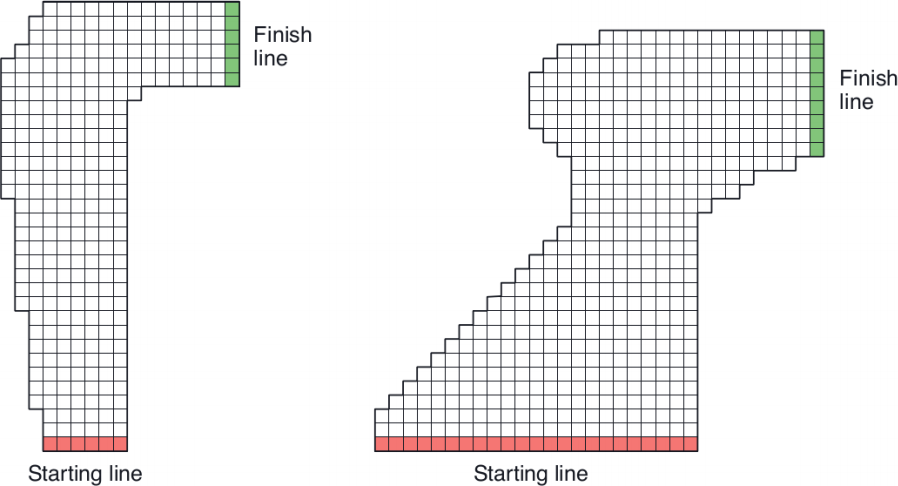
\includegraphics{3.32.png}
    \caption{A couple of right turns for the racetrack task.}
    \label{fig:4.32}
\end{figure}

\end{exercise}

% --------------------------------------------------------------------------------

\begin{solution}

ToDo!

\end{solution}

% --------------------------------------------------------------------------------

% -------------------------------------------------------------------------------- %

\begin{exercise}[Exercise 5.13]

Show the steps to derive \eqref{eq:5.14} from \eqref{eq:5.13}.
(Textbook p. 114)

\end{exercise}

% -------------------------------------------------------------------------------- %

\begin{solution}

\begin{align} \label{eq:5.14} \tag{5.14}
    \E[\rho_{t:T-1} R_{t+1}]
    =
    \E[\rho_{t:t} R_{t+1}]
\end{align}

\begin{align} \label{eq:5.13} \tag{5.13}
    \E
    \bbraces
    {
        \frac{\pi(A_k \mid S_k)}{b(A_k \mid S_k)}
    }
    \doteq
    \sum_a
        b(a \mid S_k)
        \frac{\pi(a \mid S_k)}{b(a \mid S_k)}
    =
    \sum_a
        \pi(a \mid S_k)
    =
    1
\end{align}

We use induction over $T$.
For $T = t+1$, there is nothing to prove.
Now, assume that

\begin{align*}
    \E_b[\rho_{t:t} R_{t+1}]
    =
    \E_b[\rho_{t:T-2} R_{t+1}],
\end{align*}

then

\begin{align*}
    \E_b[\rho_{t:T-1} R_{t+1}]
    & =
    \E_b
    \bbraces
    {
        \rho_{t:T-2}
        \frac{\pi(A_{T-1} \mid S_{T+1})}{b(A_{T-1} \mid S_{T+1})}
        R_{t+1}
    } \\
    & =
    \sum_a
        b(a \mid S_{T-1})
        \E_b
        \bbraces
        {
            \rho_{t:T-2}
            \frac{\pi(A_{T-1} \mid S_{T+1})}{b(A_{T-1} \mid S_{T+1})}
            R_{t+1}
            ~ \Bigg | ~
            A_{T-1} = a
        } \\
        & =
        \sum_a
            b(a \mid S_{T-1})
            \E_b
            \bbraces
            {
                \rho_{t:T-2}
                \frac{\pi(a \mid S_{T+1})}{b(a \mid S_{T+1})}
                R_{t+1}
            } \\            
        & =
        \sum_a
            b(a \mid S_{T-1})
            \frac{\pi(a \mid S_{T+1})}{b(a \mid S_{T+1})}
            \E_b
            \bbraces
            {
                \rho_{t:T-2}
                R_{t+1}
            } \\
        & =
        \underbrace
        {
            \sum_a
                \pi(a \mid S_{T-1})
        }_1
        \E_b[\rho_{t:t} R_{t+1}] \\
        & =
        \E_b[\rho_{t:t} R_{t+1}].
\end{align*}

\end{solution}

% -------------------------------------------------------------------------------- %

% -------------------------------------------------------------------------------- %

\begin{exercise}[Exercise 5.14]

Modify the algorithm for off-policy Monte Carlo control (page 111) to use the idea of the truncated weighted-average estimator \eqref{eq:5.10}.
Note that you will first need to convert this equation to action values.

\end{exercise}

% -------------------------------------------------------------------------------- %

\begin{solution}

\begin{align} \label{eq:5.10} \tag{5.10}
    V(s)
    \doteq
    \frac
    {
        \sum_{t \in \mathcal T(s)}
        \pbraces{
            (1 - \gamma)
            \sum_{h = t + 1}^{T(t) - 1}
                \gamma^{h-t-1}
                \rho_{t : h - 1}
                \bar G_{t:h}
            +
            \gamma^{T(t) - t - 1}
            \rho_{t : T(t) - 1}
            \bar G_{t : T(t)}
        }
    }{
        \sum_{t \in \mathcal T(s)}
        \pbraces{
            (1 - \gamma)
            \sum_{h = t + 1}^{T(t) - 1}
                \gamma^{h-t-1}
                \rho_{t : h - 1}
            +
            \gamma^{T(t) - t - 1}
            \rho_{t : T(t) - 1}
        }
    }
\end{align}

For $s \in \mathcal S$ and $a \in \mathcal A(x)$, let the set of time steps, where $(s, a)$ is visited, be

\begin{align*}
    \mathcal T(s, a)
    :=
    \Bbraces{t \in \N: S_t = s, A_t = a}.
\end{align*}

Now we can define \eqref{eq:5.10} for action values.

\begin{align} \label{eq:5.10'} \tag{5.10$^\prime$}
    Q(s, a)
    \doteq
    \frac
    {
        \sum_{t \in \mathcal T(s, a)}
        \pbraces{
            (1 - \gamma)
            \sum_{h = t + 1}^{T(t) - 1}
                \gamma^{h-t-1}
                \rho_{t : h - 1}
                \bar G_{t:h}
            +
            \gamma^{T(t) - t - 1}
            \rho_{t : T(t) - 1}
            \bar G_{t : T(t)}
        }
    }{
        \sum_{t \in \mathcal T(s, a)}
        \pbraces{
            (1 - \gamma)
            \sum_{h = t + 1}^{T(t) - 1}
                \gamma^{h-t-1}
                \rho_{t : h - 1}
            +
            \gamma^{T(t) - t - 1}
            \rho_{t : T(t) - 1}
        }
    }
\end{align}

In order to use an incremental implementation, we define the weights

\begin{align*}
    W_{t:h}
    \doteq
    \gamma^{h-t-1}
    \rho_{t:h-1}
    \begin{cases}
        1 - \gamma, & h < T(t), \\
        1,          & h = T(t),
    \end{cases}
    \quad
    \text{for}~
    t \in \N,
    ~\text{and}~
    h = t + 1, \dots, T(t).
\end{align*}

This lets us, analagously to \eqref{eq:5.7}, write

\begin{align} \label{eq:5.7'} \tag{5.7$^\prime$}
    Q_n(s, a)
    =
    \frac
    {
        \sum_{t \in \mathcal T_n(s, a)}
            \sum_{h=t+1}^{T(t)}
                W_{t:h} \bar G_{t:h}
    }{
        \sum_{t \in \mathcal T(s, a)}
            \sum_{h=t+1}^{T(t)}
                W_{t:h}
    },
    \quad
    n \geq 2,
\end{align}

where $\mathcal T_n(s, a)$ are the $n$ smallest elements of $\mathcal T(s, a)$.

\begin{tcolorbox}[title = {Off-policy MC control, for estimating $\pi \approx \pi_\ast$, using \eqref{eq:5.10'}}]

    Initialize, for all $s \in \mathcal S$, $a \in \mathcal A(s)$: \\
    \hspace*{0.5cm} $Q(s, a) \in \R$ (arbitrarily) \\
    \hspace*{0.5cm} $C(s, a)$ \\
    \hspace*{0.5cm} $\pi(s) \leftarrow \argmax_a Q(s, a)$ \hspace*{0.5cm} (with ties broken consistently) \\

    Loop forever (for each episode): \\
    \hspace*{0.5cm} $b \leftarrow$ any soft policy \\
    \hspace*{0.5cm} Generate an episode using $b: S_0, A_0, R_1, \dots, S_{T-1}, A_{T-1}, R_T$ \\
    \hspace*{0.5cm} Loop for each step of episode, $t = T-1, T-2, \dots, 0$: \\
    \hspace*{0.5cm} \hspace*{0.5cm} $\rho \leftarrow 1$ \\
    \hspace*{0.5cm} \hspace*{0.5cm} $\bar G \leftarrow 0$ \\
    \hspace*{0.5cm} \hspace*{0.5cm} Loop for each horizon, $h = t+1, \dots, T$: \\
    \hspace*{0.5cm} \hspace*{0.5cm} \hspace*{0.5cm} $G \leftarrow G + R_h$ \\
    \hspace*{0.5cm} \hspace*{0.5cm} \hspace*{0.5cm} $\rho \leftarrow \rho \frac{\pi(A_{h-1} \mid S_{h-1})}{b(A_{h-1} \mid S_{h-1})}$ \\
    \hspace*{0.5cm} \hspace*{0.5cm} \hspace*{0.5cm} If $h < T$, then: \\
    \hspace*{0.5cm} \hspace*{0.5cm} \hspace*{0.5cm} \hspace*{0.5cm} $C(S_t, A_t) \leftarrow C(S_t, A_t) + (1 - \gamma) \gamma^{h-t-1} \rho$ \\
    \hspace*{0.5cm} \hspace*{0.5cm} \hspace*{0.5cm} \hspace*{0.5cm} $Q(S_t, A_t) \leftarrow Q(S_t, A_t) + \frac{(1 - \gamma) \gamma^{h-t-1} \rho}{C(S_t, A_t)} (\bar G - Q(S_t, A_t))$ \\
    \hspace*{0.5cm} \hspace*{0.5cm} \hspace*{0.5cm} else: \\
    \hspace*{0.5cm} \hspace*{0.5cm} \hspace*{0.5cm} \hspace*{0.5cm} $C(S_t, A_t) \leftarrow C(S_t, A_t) + \gamma^{h-t-1} \rho$ \\
    \hspace*{0.5cm} \hspace*{0.5cm} \hspace*{0.5cm} \hspace*{0.5cm} $Q(S_t, A_t) \leftarrow Q(S_t, A_t) + \frac{\gamma^{h-t-1} \rho}{C(S_t, A_t)} (\bar G - Q(S_t, A_t))$

\end{tcolorbox}

This implementation could be modified, to be even more efficient.
In order to avoid computing $\gamma^{h-t-1}$ individually, one can use $\rho_\gamma$ instead of $\rho$.
To that end, we just substitute

\begin{itemize}
    \item $\gamma^{h-t-1}$ for $\gamma^{-1}$,
    \item $\rho_\gamma \leftarrow \rho_\gamma \frac{\pi(A_{h-1} \mid S_{h-1})}{b(A_{h-1} \mid S_{h-1})} \gamma$ for $\rho \leftarrow \rho \frac{\pi(A_{h-1} \mid S_{h-1})}{b(A_{h-1} \mid S_{h-1})}$, and the remaining
    \item $\rho_\gamma$ for $\rho$.
\end{itemize}

\end{solution}

% -------------------------------------------------------------------------------- %


\setcounter{section}{5}
\section{Temporal-Difference Learning}

% --------------------------------------------------------------------------------

\begin{exercise}[Exercise 6.1]

If $V$ changes during the episode, then \eqref{eq:6.6} only holds approximately;
what would the difference be between the two sides?
Let $V_t$ denote the array of state values used at time $t$ in the TD error \eqref{eq:6.5} and in the TD update \eqref{eq:6.2}.
Redo the derivation above to determine the additional amount that must be added to the sum of TD errors in order to equal the Monte Carlo error.
(page 121)

\end{exercise}

% --------------------------------------------------------------------------------

\begin{solution}

\begin{align} \label{eq:6.6} \tag{6.6}
    G_t - V(S_t)
    =
    \sum_{k=t}^{T-1}
        \gamma^{k-t}
        \delta_k
\end{align}

\begin{align} \label{eq:6.5} \tag{6.5}
    \delta_t
    \doteq
    R_{t+1} + \gamma V(S_{t+1}) - V(S_t)
\end{align}

\begin{align} \label{eq:6.2} \tag{6.2}
    V(S_t)
    \leftarrow
    V(S_t) + \alpha \bbraces{R_{t+1} + \gamma V(S_{t+1}) - V(S_t)}
\end{align}

Firstly, we have to adjust \eqref{eq:6.5}.

\begin{align} \label{eq:6.5'} \tag{6.5$^\prime$}
    \delta_t
    \doteq
    R_{t+1} + \gamma V_t(S_{t+1}) - V_t(S_t)
\end{align}

Then, we can redo the derivation.

\begin{align*}
    &
    G_t - V_t(S_t) \\
    & =
    R_{t+1} + \gamma G_{t+1} - V_t(S_t)
    +
    \underbrace
    {
        \gamma V_t(S_{t+1})
        -
        \gamma V_t(S_{t+1})
    }_0
    +
    \underbrace
    {
        \gamma V_{t+1}(S_{t+1})
        -
        \gamma V_{t+1}(S_{t+1})
    }_0 \\
    & =
    \delta_t
    +
    \gamma (G_{t+1} - V_{t+1}(S_{t+1}))
    +
    \gamma (V_{t+1}(S_{t+1}) - V_t(S_{t+1})) \\
    & ~ \vdots \\
    & =
    \delta_t
    +
    \gamma (\delta_{t+1} + \gamma (G_{t+2} - V_{t+2}(S_{t+2})) + \gamma (V_{t+2}(S_{t+2}) - V_{t+1}(S_{t+2})))
    +
    \gamma (V_{t+1}(S_{t+1}) - V_t(S_{t+1})) \\
    & =
    (
        \delta_t
        +
        \gamma \delta_{t+1}
    )
    +
    \gamma^2 (G_{t+2} - V_{t+2}(S_{t+2}))
    +
    (
        \gamma (V_{t+1}(S_{t+1}) - V_t(S_{t+1}))
        +
        \gamma^2 (V_{t+2}(S_{t+2}) - V_{t+1}(S_{t+2}))
    ) \\
    & ~ \vdots \\
    & =
    (
        \delta_t
        +
        \gamma \delta_{t+1}
        +
        \cdots
        +
        \gamma^{T-t-1} \delta_{T-t}
    )
    +
    \gamma^{T-t} \underbrace{(G_T - V_T(S_T))}_0 \\
    & +
    (
        \gamma (V_{t+1}(S_{t+1}) - V_t(S_{t+1}))
        +
        \gamma^2 (V_{t+2}(S_{t+2}) - V_{t+1}(S_{t+2}))
        +
        \cdots
        +
        \gamma^{T-t} (V_T(S_T) - V_{T-1}(S_T))
    ) \\
    & =
    \sum_{k=t}^{T-1}
        \gamma^{k-t} \delta_k
    +
    \sum_{k=t}^{T-1}
        \gamma^{k-t-1} (V_{k+1}(S_{k+1}) - V_k(S_{k+1})) \\
    & =
    \sum_{k=t}^{T-1}
        \gamma^{k-t}
        (
            \delta_k
            +
            \gamma (V_{k+1}(S_{k+1}) - V_k(S_{k+1}))
        )
\end{align*}

\end{solution}

% --------------------------------------------------------------------------------

% --------------------------------------------------------------------------------

\begin{exercise}[Exercise 6.8]

Show that an action-value version of \eqref{eq:6.6} holds for the action-value form of the TD error $\delta_t = R_{t+1} + \gamma Q(S_{t+1}, A_{t+1}) - Q(S_t, A_t)$, again assuming that the values don't change from step to step.

\end{exercise}

% --------------------------------------------------------------------------------

\begin{solution}

We literally only have to copy-paste the calculation yielding \eqref{eq:6.6} and replace all $V(S_k)$-s with $Q(S_k, A_k)$, for $k = t, \dots, T$.

\end{solution}

% --------------------------------------------------------------------------------

% -------------------------------------------------------------------------------- %

\begin{exercise}[Implementation Task: Windy Gridworld with King's Moves; Exercise 6.9]

Re-solve the windy gridworld assuming eight possible actions, including the diagonal moves, rather than the usual four.
How much better can you do with the extra actions?
Can you do even better by including a ninth action that causes no movement at all other than that caused by the wind?
(page 130)

\end{exercise}

% -------------------------------------------------------------------------------- %

\begin{solution}

ToDo!

\end{solution}

% -------------------------------------------------------------------------------- %

% --------------------------------------------------------------------------------

\begin{exercise}[Implementation Task: Stochastic Wind; Exercise 6.10]

Re-solve the windy gridworld task with King's moves, assuming that the effect of the wind, if there is any, is stochastic, sometimes varying by $1$ from the mean values given for each column.
That is, a third of the time you move exactly according to these values, as in the previous exercise, but also a third of the time you move one cell above that, and another third of the time you move one cell below that.
For example, if you are one cell to the right of the goal and you move left, then one-third of the time you move one cell above the goal, one-third of the time you move two cells above the goal, and one-third of the time you move to the goal.

\end{exercise}

% --------------------------------------------------------------------------------

\begin{solution}

ToDo!

\end{solution}

% --------------------------------------------------------------------------------

% --------------------------------------------------------------------------------

\begin{exercise}[Exercise 6.11]

Why is Q-learning consider an off-policy control method?

\end{exercise}

% --------------------------------------------------------------------------------

\begin{solution}

ToDo!

\end{solution}

% --------------------------------------------------------------------------------

% --------------------------------------------------------------------------------

\begin{exercise}[Exercise 6.12]

Suppose action selection is greedy.
Is Q-learning then exactly the same algorithm as Sarsa?
Will they make exactly the same action selections and weight updates?

\end{exercise}

% --------------------------------------------------------------------------------

\begin{solution}

No!
In the case of greedy action selection, one could indeed replace

\begin{align*} \label{eq:ast} \tag{$\ast$}
	Q(S, A)
	\leftarrow
	Q(S, A) + \alpha [R + \gamma Q(S^\prime, A^\prime) - Q(S, A)]
\end{align*}

by

\begin{align*}
	Q(S, A)
	\leftarrow
	Q(S, A) + \alpha \bbraces{R + \gamma \max _a Q(S^\prime, a) - Q(S, A)}
\end{align*}

and expect the algorithms to operate the same in the first loop instance.
However, in order for them to do so in the future, one should include, in Sarsa,

\begin{displayquote}
	Choose $A^\prime$ from $S^\prime$ using policy derived from $Q$ (greedy)
\end{displayquote}

after \eqref{eq:ast}.
Then, both Sarsa and Q-learning will both be on-policy, i.e. they use the same policy for generating samples, as they do for updating $Q$.

\end{solution}

% --------------------------------------------------------------------------------

% -------------------------------------------------------------------------------- %

\begin{exercise}[Exercise 6.13]

What are the update equations for Double Expected Sarsa with an $\epsilon$-greedy target policy?

\end{exercise}

% -------------------------------------------------------------------------------- %

\begin{solution}

They are

\begin{align*}
    Q_i(S_t, A_t)
    \leftarrow
    Q_i(S_t, A_t) + \alpha \bbraces{R_{t+1} + \gamma \sum_a \pi(a \mid S_{t+1}) Q_i(S_{t+1}, a) - Q_i(S_t, A_t)},
    \quad
    \text{where}
    \quad
    i = 1, 2,
\end{align*}

and $\pi$ is $\epsilon$-greedy w.r.t. $Q_1 + Q_2$, i.e.

\begin{align*}
    \pi(a \mid s)
    =
    \frac{\epsilon}{|\mathcal A(s)|}
    +
    \begin{cases}
        1 - \epsilon, & a = a^\ast, \\
        0,            & \text{else},
    \end{cases}
    \quad
    \text{for}
    \quad
    s \in \mathcal S,
    \quad
    \text{where}
    \quad
    a^\ast = \argmax_a (Q_1(s, a) + Q_2(s, a)).
\end{align*}

\end{solution}

% -------------------------------------------------------------------------------- %


\printbibliography

\end{document}
